\capitolo{Controlli Automatici}
Ripasso di controlli automatici con focus su: Trasformata di Laplace; Diagrammi di Bode; Luogo delle radici; Criteri di stabilità; Analisi di sistemi nel tempo e in frequenza.

\sezione{Trasformata di Laplace}
La trasformata di Laplace bilatera del segnale $x:\mathbb{R} \rightarrow \mathbb{C}$ è la funzione $X:\mathbb{C} \rightarrow \mathbb{C}$, $s \rightarrow X(s) := \int^\infty_{-\infty} x(t)e^{-st} dt $, per ogni $s=\sigma + j\omega\in \mathbb{C}$ per cui l'integrale converge. Si denota come $\laplace{x(t)} = X(s)$.

\sottosezione{Proprietà}
Principali proprietà della trasformata di Laplace.
\begin{itemize}
    \item Traslazione in t: $\laplace{x(t+\beta)} = e^{s\beta}X(s)$
    \item Traslazione in s: $\laplace{e^{s_0t}x(t)} = X(s-s_0)$
    \item Cambio di scala: $\laplace{x(at)} = \frac{1}{\abs{a}}X(\frac{s}{a})$
    \item Derivata in s: $\laplace{tx(t)}=-\derivata{X(s)}{s}$
    \item Convoluzione: $\laplace{v(t)*w(t)} = V(s)W(s)$
    \item Integrazione in t: $\laplace{\int^t_{-\infty} x(\tau) d\tau }=\frac{X(s)}{s}$
    \item Antritrasformata di Laplace: $x(t)=\frac{1}{2\pi} \int^\infty_{-\infty}X(\sigma+j\omega) e^{(\sigma+j\omega)t} d\omega$
    \item Derivata in t: $\laplace{\derivata{x(t)}{t}} = s X(s)$
\end{itemize}

%% valutare di copiarne altre da appunti di controlli

\sottosezione{Funzione di Trasferimento}
%% Inserire definizione di funzione di trasferimento su appunti

\sezione{Diagrammi di Bode}
Per rappresentare le risposte armoniche si utilizza una coppia di diagrammi detti di Bode:
\begin{enumerate}
    \item $\abs{G(j\omega)}$ funzione di $\omega$
    \item $\arg{G(j\omega)}$ funzione di $\omega$
\end{enumerate}

Sono diagrammi semilogaritmici (anche logaritmici) utili per rappresentare ampi intervalli di pulsazioni e quindi permettono di osservare facilmente amplificazioni e attenuazioni.

\sottosottosezione{Decibel}
Il decibel, adimensionale perché indica rapporti di grandezze equivalenti dimensionalmente, è definito per le ampiezze come $G_{dB} = 20\log_{10}{\abs{H(j\omega)}}$. Il decibel è usato nei diagrammi di Bode per rappresentare le ampiezze delle risposte in esame.

\sottosottosezione{Fasi}
Le fasi $\arg{1+j\omega \tau}=\arctan{\omega \tau}$, 

\sottosottosezione{Regole di tracciamento}
Nel caso di ampiezze:
\begin{enumerate}
    \item Costanti: rette orizzontali
    \item Poli: Per ogni ordine n hanno pendenza di $-n\cdot 20dB$ per decade 
    \item Zeri: Per ogni ordine n hanno pendenza di $+n\cdot 20dB$ per decade
\end{enumerate}

Nel caso di fasi:
\begin{enumerate}
    \item Costanti: $0 rd$
    \item Poli: Per ogni ordine n hanno pendenza di $-n\cdot \frac{\pi}{4}$ per decade, per una durata totale di due decadi
    \item Zeri: Per ogni ordine n hanno pendenza di $n\cdot \frac{\pi}{4}$ per decade, per una durata totale di due decadi
\end{enumerate}

\sezione{Luogo delle radici}
Strumento che consente di valutare graficamente l'andamento delle radici del denominatore di una funzione di trasferimento ottenuta mettendo in retroazione il blocco di andata costituito da $G(s)$ e blocco proporzionale $K$, e il blocco di retroazione $1$. 
Definito $G(s)=\frac{N(s)}{D(s)}$, monico e coprimo; il polinomio caratteristico del sistema in retroazione unitaria è dato da $D(s) + K N(s) = 0$, e rappresenta i poli di $W(s)=\frac{K N(s)}{D(s) + K N(s)}$. Al variare di $K$, con il luogo delle radici, è possibile analizzare la posizione dei poli del sistema a catena chiusa $W(s)$.

\sottosezione{Step}
\begin{enumerate}[label=\roman*.]
    \item Funzione di trasferimento del sistema ad anello aperto: Scrivere la funzione di trasferimento del sistema ad anello aperto $G(s)H(s)$, dove: $G(s)H(s)=N(s)D(s)$; $N(s)$: numeratore del sistema; $D(s)$: denominatore del sistema. Questa funzione è solitamente espressa in termini di poli e zeri del sistema.

    \item Trovare i poli e gli zeri: Determinare i poli (tali che $D(s)=0$) e gli zeri (tali che $N(s)=0$) del sistema ad anello aperto. I poli (disegnati solitamente con una "x") determinano le posizioni iniziali delle traiettorie del luogo delle radici, mentre gli zeri (disegnati solitamente con un "o") ne determinano le destinazioni finali.

    \item Determinare la quantità di traiettorie: Il numero di rami (traiettorie del luogo delle radici) è uguale al numero di poli del sistema ad anello aperto. Ogni ramo inizia da un polo del sistema e tende verso uno zero del sistema, o verso l'infinito se ci sono più poli che zeri.

    \item Trovare l'asse reale coinvolto nel luogo delle radici: Determinare i tratti dell'asse reale che fanno parte del luogo delle radici. Un segmento sull'asse reale fa parte del luogo delle radici se alla sua destra ci sono un numero dispari di poli e zeri.

    \item Determinare i punti di separazione e arrivo (Asintoti): Se ci sono più poli che zeri, calcolare gli asintoti delle traiettorie del luogo delle radici, che indicano dove i rami tendono all'infinito. Gli asintoti possono essere trovati con: $\textup{Angoli degli asintoti}=\frac{(2k+1)\pi}{n-m}$
    Dove $n$ è il numero di poli, $m$ è il numero di zeri; $k=0,1,2,…$, di cui devono essere indagati tutti i valori fino a quando non si giunga ad una ripetizione degli angoli. 
    Il punto di intersezione con l'asse reale è dato da: $\sigma_a=\frac{\sum \textup{Poli}-\sum \textup{Zeri}}{n-m}$

    \item Trovare i punti di rottura (breakaway) sull'asse reale: Se due o più rami si uniscono o si separano sull'asse reale, questo avviene in punti detti punti di rottura. Per determinare tali punti, risolvere la derivata della funzione caratteristica del sistema: $\derivata{​(1+KG(s)H(s))}{s}=0$, o in modo empirico calcolando \( \sum^m_1\frac{1}{\sigma - z_i} = \sum^n_1 \frac{1}{\sigma-p_i} \) dove \( z_i \) è lo zero e \( p_i \) il polo, questo restituisce la coordinata sull'asse reale del punto studiato.

    \item Calcolare gli angoli di partenza e arrivo: Determinare l'angolo di partenza per i rami che si staccano dai poli complessi e l'angolo di arrivo per quelli che si avvicinano agli zeri complessi. Questi angoli sono calcolati con le equazioni basate sulla posizione relativa di poli e zeri complessi rispetto al polo o allo zero in questione.

    \item Determinare i punti di intersezione con l'asse immaginario (criterio di Routh-Hurwitz): Verificare se i rami del luogo delle radici attraversano l'asse immaginario. Questo può essere fatto utilizzando il criterio di Routh-Hurwitz per trovare i valori di \( K \) per cui il sistema ha poli con parte reale nulla (ossia poli puramente immaginari).

    \item Tracciare il luogo delle radici: Con tutte le informazioni raccolte, tracciare il diagramma del luogo delle radici:
    \begin{enumerate}
        \item Parti dai poli ad anello aperto.
        \item Disegna i rami lungo l'asse reale e seguendo gli asintoti.
        \item Mostra come i rami si avvicinano agli zeri o tendono all'infinito.
        \item Indica chiaramente i punti di rottura, intersezioni con l'asse immaginario e altri dettagli chiave.
    \end{enumerate}
\end{enumerate}

\sottosezione{Proprietà extra}
\begin{itemize}
    \item Per trovare un punto nel luogo della radici, noti gli angoli tra ciascuno zero e quel punto \( \theta_z \), e tra angoli tra ciascun polo e quel punto \( \theta_p \): \( \sum \theta_z - \sum \theta_p = -180° \).
    \item Lo smorzamento nel diagramma corrisponde a un angolo \( \theta = \cos^{-1} (\psi) \).
    \item Sussiste una relazione tra il guadagno ad anello aperto e \( K_\text{tot} = \frac{1}{\abs{G_\text{open}H}} = \frac{\Pi L_{p,i}}{\Pi L_{z,i}} \) con \( L_p \) e \( L_z \) lunghezze dei poli/zeri, ossia distanza tra polo/zero e punto di interesse. Se non ci sono poli o zeri, vanno posti a 1.
\end{itemize}

\sottosezione{Esempio}
Per esempio fare il luogo delle radici di $G(s) = \frac{s + 3}{(s + 1)(s + 5)(s + 10)}$ risulta nel seguente grafico:
\begin{figure}[h]
    \centering
    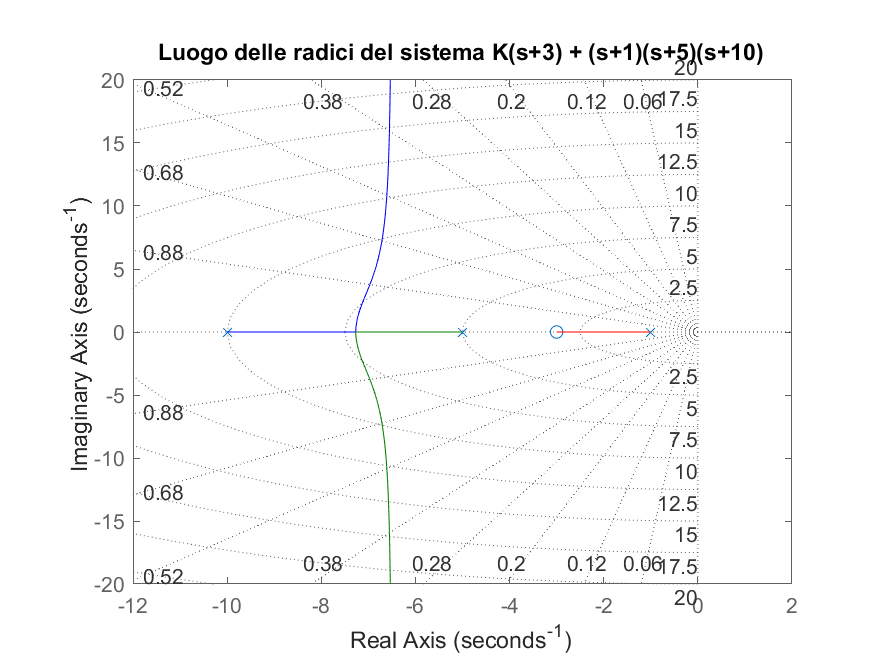
\includegraphics[width=0.4\textwidth]{Immagini/luogo_delle_radici.png}
\end{figure}

%% Rivedere parte su luogo delle radici